%%%%%%%%%%%%%%%%%%%%%%%%%%%%%%%%%%%%%%%%%%%%%%%%%%%%%%%%%%%%%%%%%%%%%%%%%%%%%%%%%%%%%%%%%%%%%%%%%%%%%%%%%%%%%%%%%%%%%%%%%%%%%%%%%%%%%%%%%%%%%%%%%%%%%%%%%%%%%%%%%%%
% Written By Michael Brodskiy
% Class: Modern Physics
% Professor: Q. Yan
%%%%%%%%%%%%%%%%%%%%%%%%%%%%%%%%%%%%%%%%%%%%%%%%%%%%%%%%%%%%%%%%%%%%%%%%%%%%%%%%%%%%%%%%%%%%%%%%%%%%%%%%%%%%%%%%%%%%%%%%%%%%%%%%%%%%%%%%%%%%%%%%%%%%%%%%%%%%%%%%%%%

\include{Includes.tex}

\title{The Particle-Like Properties of Electromagnetic Waves}
\date{\today}
\author{Michael Brodskiy\\ \small Professor: Q. Yan}

\begin{document}

\maketitle

\newpage

\tableofcontents

\newpage

\begin{itemize}

    \section{Review of Electromagnetic Waves}

  \item Reviewing the nature of light (or electromagnetic waves)

    \begin{itemize}

      \item A plane wave

        \begin{itemize}

          \item A plane wave traveling in the positive x direction:

            $$\left\{\begin{array}{c} \vec{E}=\vec{E}_o\sin(kx-\omega t)\\\vec{B}=\vec{B}_o\sin(kx-\omega t) \end{array}$$

            \item The direction of energy transport would be $\vec{E}\times\vec{B}$

            \item $|\vec{E}|$ and $|\vec{B}|$ are constant at a given $t$

            \item The power, $P$, of the wave:

              $$P=\frac{E}{\Delta t}=\frac{1}{\mu_oc}E_o^2A\sin^2(kx-\omega t)$$

            \item Two important features:

              \begin{enumerate}

                \item Intensity (average power per unit area) is proportional to $E_o^2$

                  $$P_{avg}=\int_0^T P(t)\,dt$$

                \item  The intensity of the system fluctuates with time

                  $$\frac{P_{avg}}{A}$$

              \end{enumerate}

        \end{itemize}

      \item A spherical wave

        \begin{itemize}

          \item Spreads out uniformly along the three axis

        \end{itemize}

    \end{itemize}

    \section{The Photoelectric Effect}

  \item Experiment performed by Heinrich Hertz (1887)

  \item When a metal surface is illuminated, light electrons can be emitted from the surface

  \item The Experiment:

    \begin{itemize}

      \item Connect emitter and collector to an external circuit

      \item Apply a negative potential to the circuit collector

      \item Increase the potential difference ($(-V)-(+V)$) to be more negative

      \item At some point, even the most energetic electrons do not have enough kinetic energy to reach the collector

      \item The maximum kinetic energy to reach the collector with the stopping voltage, $V_s$, is:

        $$K_{max}=eV_s$$

    \end{itemize}

    \begin{figure}[h!]
      \centering
      \tikzset{every picture/.style={line width=0.75pt}} %set default line width to 0.75pt        

\begin{tikzpicture}[x=0.75pt,y=0.75pt,yscale=-1,xscale=1]
%uncomment if require: \path (0,642); %set diagram left start at 0, and has height of 642

%Shape: Boxed Line [id:dp5098624474614848] 
\draw    (150,108.29) -- (150,249.71) ;
%Shape: Boxed Line [id:dp4883126832478788] 
\draw    (452,108.29) -- (452,249.71) ;
%Shape: Battery [id:dp21984735994344673] 
\draw   (453,249.71) -- (316.65,249.71) (286.35,279.71) -- (286.35,219.71) (286.35,249.71) -- (150,249.71) (328.77,264.71) -- (316.65,264.71) -- (316.65,234.71) -- (328.77,234.71) -- (328.77,264.71) -- cycle ;
%Straight Lines [id:da07825154591470551] 
\draw    (240.42,108.29) -- (150,108.29) ;
%Straight Lines [id:da10296831027951714] 
\draw    (452,108.29) -- (361.58,108.29) ;
%Shape: Rectangle [id:dp45994932364238905] 
\draw   (240,78) -- (262,78) -- (262,139) -- (240,139) -- cycle ;
%Straight Lines [id:da8703604595072303] 
\draw    (361.58,37.58) -- (361.58,179) ;
%Straight Lines [id:da37814010167699585] 
\draw  [dash pattern={on 0.84pt off 2.51pt}]  (262.42,101.29) -- (362.42,1.29) ;
%Straight Lines [id:da7637770505032595] 
\draw  [dash pattern={on 0.84pt off 2.51pt}]  (262.42,108.29) -- (362.42,8.29) ;
%Straight Lines [id:da7153723628671289] 
\draw  [dash pattern={on 0.84pt off 2.51pt}]  (261.42,95.29) -- (361.42,-4.71) ;
%Straight Lines [id:da04025150844205161] 
\draw    (262.42,108.29) -- (298.58,108.29) ;
\draw [shift={(300.58,108.29)}, rotate = 180] [color={rgb, 255:red, 0; green, 0; blue, 0 }  ][line width=0.75]    (10.93,-3.29) .. controls (6.95,-1.4) and (3.31,-0.3) .. (0,0) .. controls (3.31,0.3) and (6.95,1.4) .. (10.93,3.29)   ;

% Text Node
\draw (284.35,282.71) node [anchor=north east] [inner sep=0.75pt]   [align=left] {$\displaystyle +V$};
% Text Node
\draw (330.77,267.71) node [anchor=north west][inner sep=0.75pt]   [align=left] {$\displaystyle -V$};
% Text Node
\draw (238,75) node [anchor=south east] [inner sep=0.75pt]   [align=left] {Emitter};
% Text Node
\draw (300.58,111.29) node [anchor=north] [inner sep=0.75pt]   [align=left] {$\displaystyle e^{-}$};


\end{tikzpicture}

      \caption{Set up of the Photoelectric Effect Experiment}
      \label{fig:1}
    \end{figure}

    \begin{itemize}

      \item The classical picture: The energy of light with intensity $I$ is absorbed by electrons, $E_{light} > E_{binding}$, $e$ is released


      \item What does the classical wave theory predict?

        \begin{enumerate}

          \item The maximum kinetic energy of the electrons, $K_{max}$, is proportional to the intensity of light

          \item The effect occurs for light with any frequency or wavelength

          \item $e^-$ are released after a finite $\Delta t$

        \end{enumerate}

    \end{itemize}

  \item Experimental Results

    \begin{enumerate}

      \item For a fixed $f$ or $\lambda$, $K_{max}$ is independent of the intensity of light

      \item The effect occurs only if $f>f_{\text{cutoff}}$

      \item The first electrons are emitted almost instantaneously ($<10^{-9}[\si{\second}]$)

    \end{enumerate}

    \begin{itemize}

      \item This means everything that classical wave theory predicted was essentially incorrect

    \end{itemize}

  \item The Quantum Theory of the Photoelectric Effect

    \begin{itemize}

      \item Developed by Albert Einstein (in 1905), based on Max Planck's idea explaining thermal radiation

      \item Assumptions:

        \begin{itemize}

          \item The energy of electromagnetic waves is not continuously distributed

          \item The energy is concentrated in localized bands or ``quanta''

          \item This quanta is called ``photon''

        \end{itemize}

      \item The energy of a photon is $\boxed{E=hf}$, where $h$ is Planck's constant, and $f$ is the frequency

        $$\boxed{f=\frac{c}{\lambda}\Rightarrow E=\frac{hc}{\lambda}}$$

      \item Photons travel at speed $c$, and are technically massless, so:

        $$\boxed{p=\frac{E}{c}=\frac{h}{\lambda}}$$

      \item If $E=hf>\phi$, then photoelectrons are released; $E$ is the photon energy, and $\phi$ is the work function

      \item The kinetic energy of the electron is:

        $$\boxed{K_{max}=hf-\phi}$$

      \item Evidently, the intensity is not relevant; a larger intensity would mean more photons in a unit area, which means more electrons released; this means there is more current.

    \end{itemize}

  \item In 1915, Robert Millikan performed an experiment (won 1923 Nobel Prize)

    \begin{itemize}

      \item Determined Planck's constant ($h=6.57\cdot10^{-34}\si{\joule\second}$)

      \item Fairly accurate, modern calculations found $h=6.626\cdot10^{-34} \si{\joule\second}$

    \end{itemize}

  \item The Photoelectric Effect Formula:

    $$\boxed{\lambda_c=\frac{hc}{\phi}}$$

    \begin{itemize}

      \item Where $\lambda_c$ is the cutoff wavelength, $h$ is Planck's constant, and $\phi$ is the work function

    \end{itemize}

    \section{Compton Effect}

  \item From classical physics (optics), $\lambda_1=\lambda_2$

    \begin{figure}[h!]
      \centering
      \tikzset{every picture/.style={line width=0.75pt}} %set default line width to 0.75pt        

\begin{tikzpicture}[x=0.75pt,y=0.75pt,yscale=-1,xscale=1]
%uncomment if require: \path (0,642); %set diagram left start at 0, and has height of 642

%Shape: Rectangle [id:dp4884979270157479] 
\draw   (152,146) -- (432,146) -- (432,264) -- (152,264) -- cycle ;
%Straight Lines [id:da09234309558155318] 
\draw [line width=1.5]  [dash pattern={on 1.69pt off 2.76pt}]  (147,62) -- (289.53,144.01) ;
\draw [shift={(293,146)}, rotate = 209.91] [fill={rgb, 255:red, 0; green, 0; blue, 0 }  ][line width=0.08]  [draw opacity=0] (11.61,-5.58) -- (0,0) -- (11.61,5.58) -- cycle    ;
%Straight Lines [id:da17812306023892588] 
\draw [line width=1.5]  [dash pattern={on 1.69pt off 2.76pt}]  (293,146) -- (435.53,63.99) ;
\draw [shift={(439,62)}, rotate = 150.09] [fill={rgb, 255:red, 0; green, 0; blue, 0 }  ][line width=0.08]  [draw opacity=0] (11.61,-5.58) -- (0,0) -- (11.61,5.58) -- cycle    ;
%Straight Lines [id:da6647955313115745] 
\draw [line width=1.5]  [dash pattern={on 1.69pt off 2.76pt}]  (293,146) -- (357.02,258.52) ;
\draw [shift={(359,262)}, rotate = 240.36] [fill={rgb, 255:red, 0; green, 0; blue, 0 }  ][line width=0.08]  [draw opacity=0] (11.61,-5.58) -- (0,0) -- (11.61,5.58) -- cycle    ;

% Text Node
\draw (149,59) node [anchor=south west] [inner sep=0.75pt]   [align=left] {Light Beam 1 ($\displaystyle \lambda _{1}$)};
% Text Node
\draw (361,265) node [anchor=north west][inner sep=0.75pt]   [align=left] {Light Beam 2};
% Text Node
\draw (441,65) node [anchor=north west][inner sep=0.75pt]   [align=left] {Reflection ($\displaystyle \lambda _{v}$)};


\end{tikzpicture}

      \caption{Classical Reflection of a Light Beam}
      \label{fig:2}
    \end{figure}

  \item There will be a scattering process (Figure \ref{fig:3})

    \begin{itemize}

      \item An incident photon ($E,p$) collides with a stationary electron

      \item The photon ($E',p'$) is scattered with angle $\theta$

      \item The electron ($E_e,p_e$) is scattered with angle $\phi$

    \end{itemize}

    \begin{figure}[h!]
      \centering
      \tikzset{every picture/.style={line width=0.75pt}} %set default line width to 0.75pt        

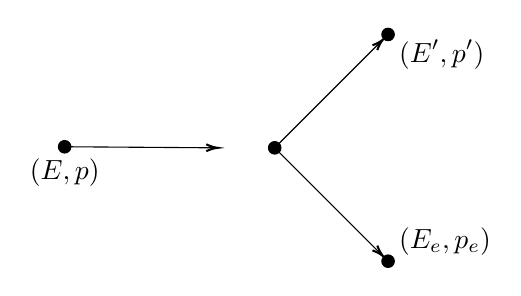
\begin{tikzpicture}[x=0.75pt,y=0.75pt,yscale=-.5,xscale=.5]
%uncomment if require: \path (0,642); %set diagram left start at 0, and has height of 642

%Straight Lines [id:da3983605421864147] 
\draw    (79.29,166) -- (218.71,166.99) ;
\draw [shift={(220.71,167)}, rotate = 180.41] [color={rgb, 255:red, 0; green, 0; blue, 0 }  ][line width=0.75]    (10.93,-3.29) .. controls (6.95,-1.4) and (3.31,-0.3) .. (0,0) .. controls (3.31,0.3) and (6.95,1.4) .. (10.93,3.29)   ;
%Shape: Circle [id:dp6842291847436652] 
\draw  [fill={rgb, 255:red, 0; green, 0; blue, 0 }  ,fill opacity=1 ] (67.29,166) .. controls (67.29,162.69) and (69.98,160) .. (73.29,160) .. controls (76.6,160) and (79.29,162.69) .. (79.29,166) .. controls (79.29,169.31) and (76.6,172) .. (73.29,172) .. controls (69.98,172) and (67.29,169.31) .. (67.29,166) -- cycle ;
%Shape: Circle [id:dp1597637002944694] 
\draw  [fill={rgb, 255:red, 0; green, 0; blue, 0 }  ,fill opacity=1 ] (269.71,167) .. controls (269.71,163.69) and (272.4,161) .. (275.71,161) .. controls (279.02,161) and (281.71,163.69) .. (281.71,167) .. controls (281.71,170.31) and (279.02,173) .. (275.71,173) .. controls (272.4,173) and (269.71,170.31) .. (269.71,167) -- cycle ;
%Straight Lines [id:da615761383513229] 
\draw    (275.71,167) -- (378.54,64.17) ;
\draw [shift={(379.95,62.76)}, rotate = 135] [color={rgb, 255:red, 0; green, 0; blue, 0 }  ][line width=0.75]    (10.93,-3.29) .. controls (6.95,-1.4) and (3.31,-0.3) .. (0,0) .. controls (3.31,0.3) and (6.95,1.4) .. (10.93,3.29)   ;
%Straight Lines [id:da4299869565163963] 
\draw    (275.71,167) -- (378.54,269.83) ;
\draw [shift={(379.95,271.24)}, rotate = 225] [color={rgb, 255:red, 0; green, 0; blue, 0 }  ][line width=0.75]    (10.93,-3.29) .. controls (6.95,-1.4) and (3.31,-0.3) .. (0,0) .. controls (3.31,0.3) and (6.95,1.4) .. (10.93,3.29)   ;
%Shape: Circle [id:dp7940631677488701] 
\draw  [fill={rgb, 255:red, 0; green, 0; blue, 0 }  ,fill opacity=1 ] (378.95,57.76) .. controls (378.95,54.44) and (381.64,51.76) .. (384.95,51.76) .. controls (388.27,51.76) and (390.95,54.44) .. (390.95,57.76) .. controls (390.95,61.07) and (388.27,63.76) .. (384.95,63.76) .. controls (381.64,63.76) and (378.95,61.07) .. (378.95,57.76) -- cycle ;
%Shape: Circle [id:dp9447740865983771] 
\draw  [fill={rgb, 255:red, 0; green, 0; blue, 0 }  ,fill opacity=1 ] (378.95,276.24) .. controls (378.95,272.93) and (381.64,270.24) .. (384.95,270.24) .. controls (388.27,270.24) and (390.95,272.93) .. (390.95,276.24) .. controls (390.95,279.56) and (388.27,282.24) .. (384.95,282.24) .. controls (381.64,282.24) and (378.95,279.56) .. (378.95,276.24) -- cycle ;

% Text Node
\draw (73.29,175) node [anchor=north] [inner sep=0.75pt]   [align=left] {($\displaystyle E,p$)};
% Text Node
\draw (392.95,60.76) node [anchor=north west][inner sep=0.75pt]   [align=left] {($\displaystyle E',p'$)};
% Text Node
\draw (392.95,273.24) node [anchor=south west] [inner sep=0.75pt]   [align=left] {($\displaystyle E_{e} ,p_{e}$)};


\end{tikzpicture}

      \caption{Collision of Photon and Electron}
      \label{fig:3}
    \end{figure}

  \item Conservation of Energy and Momentum

    \begin{itemize}

      \item $E_i=E_f\Rightarrow E+m_ec^2=E'+E_e$

      \item Momentum

        \begin{itemize}

          \item $p_{xi}=p_{xf}\Rightarrow p=p'\cos(\theta)+p_e\cos(\phi)$

          \item $p_{yi}=p_{yf}\Rightarrow 0=p'\sin(\theta)+p_e\sin(\phi)$

        \end{itemize}
        
      \item Conservation Laws:

        $$\boxed{E-E'=E_e-m_ec^2=K_e}$$

      \item After a lot of algebra and formula manipulations, we get:

        $$\boxed{\lambda'-\lambda=\frac{h}{m_ec}\left( 1-\cos(\theta) \right)}$$

      \item $\lambda'$ is the wavelength of the scattered photon, $\lambda$ is the wavelength of the incident photon, and $\dfrac{h}{m_ec}$ is the Compton wavelength (approximately $.002426[\si{\nano\meter}]$)

      \item Thus, after scattering, we know $\lambda' \geq \lambda$

        $$\lambda'-\lambda = \left\{\begin{array}{c c} 0, & \text{when }\theta = 0\\\\ \dfrac{2h}{m_ec}, & \text{when }\theta=180 \end{array}$$

        \item Electron has maximum energy when $\theta$ is closer to 180, and minimum energy when $\theta$ is closer to 0

        \item The experiment was done by Arthur Compton in 1923

          \begin{itemize}

            \item A beam of x-rays of wavelength $\lambda$ is incident on carbon (``nearly free'' electrons); measured the scattered x-ray intensity as a function of $\theta$

          \end{itemize}

    \end{itemize}

    \section{Thermal Radiation}

  \item The total intensity $\left( \displaystyle \int I(\lambda)\,d\lambda \right)$ increases as $T$ is increased

  \item Stefan's Law: $I=\sigma T^4$

  \item $\lambda_{\text{max}}$ decreases as $T$ increases

  \item Wien's Displacement: $\lambda_{\text{max}}T=2.9\cdot10^{-3}[\si{\meter\kelvin}]$
    
  \item Classical theory outline of $I(\lambda)$ vs. $\lambda$:

    \begin{itemize}

      \item A box is filled with an EM standing wave (black body)

      \item The number of standing waves with a wavelength between $\lambda$ and $\lambda+d\lambda$ is:

        $$N(\lambda)\,d\lambda = \dfrac{8\pi V}{\lambda^4}\,d\lambda$$

      \item Each standing wave carries $E_{avg}$

        $$E_{avg}=k_BT$$

      \item Energy Density (\# of standing waves per volume):

        $$u(\lambda)\,d\lambda=\dfrac{8\pi}{\lambda^4}k_BT\,d\lambda$$
        $$I(\lambda)=\frac{c}{4}u(\lambda)$$
        $$\boxed{I(\lambda)=\dfrac{2\pi c}{\lambda^4}k_BT}$$

      \item This is known as the Rayleigh-Jones formula

        \begin{itemize}

          \item It approaches the correct intensity at large wavelengths

          \item Fails at small wavelengths

          \item Known as the ultraviolet catastrophe

        \end{itemize}

    \end{itemize}

  \item Quantum Theory of Thermal Radiation

    \begin{itemize}

      \item The theory was proposed by Max Planck in 1900

      \item What was needed? $u(\lambda)\to 0$ when $\lambda \to 0$

      \item An oscillating atom can absorb or emit energy only in discrete bundles

        \begin{figure}[h!]
          \centering
          \tikzset{every picture/.style={line width=0.75pt}} %set default line width to 0.75pt        

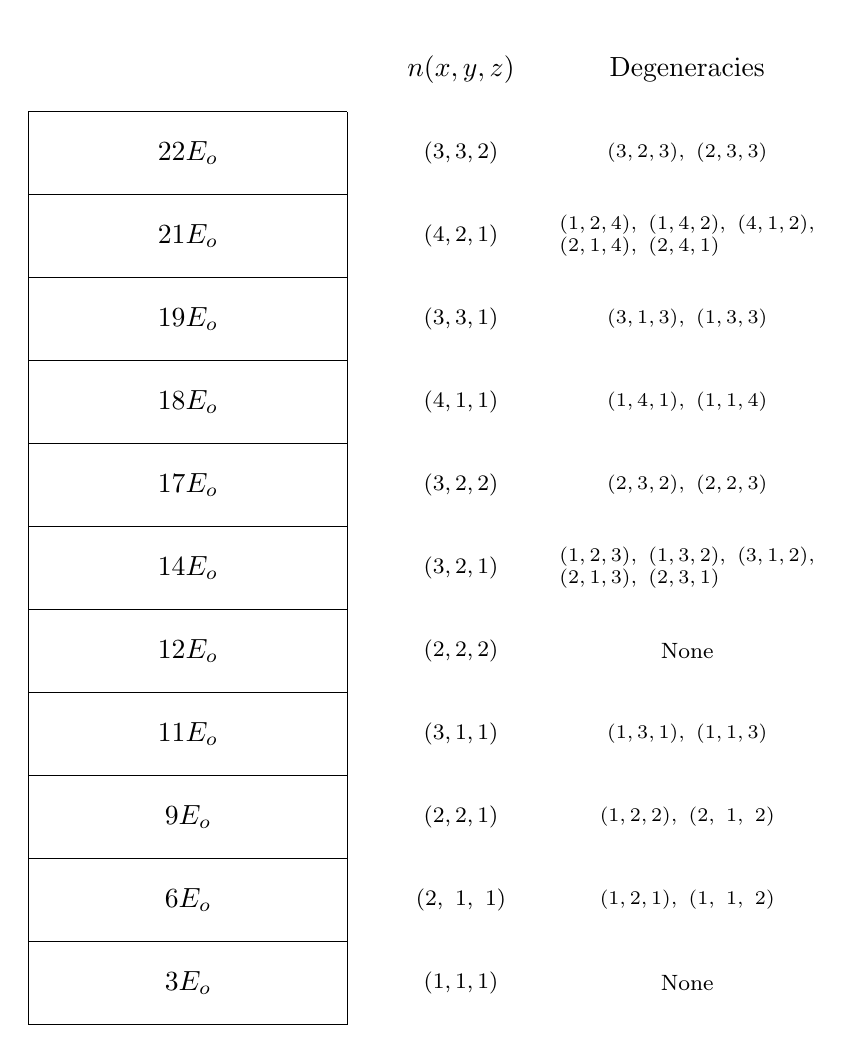
\begin{tikzpicture}[x=0.75pt,y=0.75pt,yscale=-1,xscale=1]
%uncomment if require: \path (0,538); %set diagram left start at 0, and has height of 538

%Shape: Rectangle [id:dp7431820249349796] 
\draw  [color={rgb, 255:red, 255; green, 255; blue, 255 }  ,draw opacity=1 ][fill={rgb, 255:red, 255; green, 255; blue, 255 }  ,fill opacity=1 ] (253,87) -- (362,87) -- (362,127) -- (253,127) -- cycle ;
%Shape: Rectangle [id:dp4619815785817558] 
\draw  [color={rgb, 255:red, 255; green, 255; blue, 255 }  ,draw opacity=1 ][fill={rgb, 255:red, 255; green, 255; blue, 255 }  ,fill opacity=1 ] (253,127) -- (362,127) -- (362,167) -- (253,167) -- cycle ;
%Shape: Rectangle [id:dp3359362966762425] 
\draw  [color={rgb, 255:red, 255; green, 255; blue, 255 }  ,draw opacity=1 ][fill={rgb, 255:red, 255; green, 255; blue, 255 }  ,fill opacity=1 ] (253,167) -- (362,167) -- (362,207) -- (253,207) -- cycle ;
%Shape: Rectangle [id:dp5119516390611945] 
\draw  [color={rgb, 255:red, 255; green, 255; blue, 255 }  ,draw opacity=1 ][fill={rgb, 255:red, 255; green, 255; blue, 255 }  ,fill opacity=1 ] (253,207) -- (362,207) -- (362,247) -- (253,247) -- cycle ;
%Shape: Rectangle [id:dp00577409558737596] 
\draw  [color={rgb, 255:red, 255; green, 255; blue, 255 }  ,draw opacity=1 ][fill={rgb, 255:red, 255; green, 255; blue, 255 }  ,fill opacity=1 ] (253,247) -- (362,247) -- (362,287) -- (253,287) -- cycle ;
%Shape: Rectangle [id:dp9392024809985304] 
\draw  [color={rgb, 255:red, 255; green, 255; blue, 255 }  ,draw opacity=1 ][fill={rgb, 255:red, 255; green, 255; blue, 255 }  ,fill opacity=1 ] (253,287) -- (362,287) -- (362,327) -- (253,327) -- cycle ;
%Shape: Rectangle [id:dp36507090012453736] 
\draw  [color={rgb, 255:red, 255; green, 255; blue, 255 }  ,draw opacity=1 ][fill={rgb, 255:red, 255; green, 255; blue, 255 }  ,fill opacity=1 ] (253,327) -- (362,327) -- (362,367) -- (253,367) -- cycle ;
%Shape: Rectangle [id:dp3845863388878359] 
\draw  [color={rgb, 255:red, 255; green, 255; blue, 255 }  ,draw opacity=1 ][fill={rgb, 255:red, 255; green, 255; blue, 255 }  ,fill opacity=1 ] (253,367) -- (362,367) -- (362,407) -- (253,407) -- cycle ;
%Shape: Rectangle [id:dp08289501558521084] 
\draw  [color={rgb, 255:red, 255; green, 255; blue, 255 }  ,draw opacity=1 ][fill={rgb, 255:red, 255; green, 255; blue, 255 }  ,fill opacity=1 ] (253,407) -- (362,407) -- (362,447) -- (253,447) -- cycle ;
%Shape: Rectangle [id:dp30336721777460673] 
\draw  [color={rgb, 255:red, 255; green, 255; blue, 255 }  ,draw opacity=1 ][fill={rgb, 255:red, 255; green, 255; blue, 255 }  ,fill opacity=1 ] (253,47) -- (362,47) -- (362,87) -- (253,87) -- cycle ;
%Shape: Rectangle [id:dp33732499056647836] 
\draw   (99,407) -- (253,407) -- (253,447) -- (99,447) -- cycle ;
%Shape: Rectangle [id:dp11504885678961019] 
\draw   (99,367) -- (253,367) -- (253,407) -- (99,407) -- cycle ;
%Shape: Rectangle [id:dp469041150289242] 
\draw   (99,327) -- (253,327) -- (253,367) -- (99,367) -- cycle ;
%Shape: Rectangle [id:dp5969911762901989] 
\draw   (99,287) -- (253,287) -- (253,327) -- (99,327) -- cycle ;
%Shape: Rectangle [id:dp6587152869266266] 
\draw   (99,247) -- (253,247) -- (253,287) -- (99,287) -- cycle ;
%Shape: Rectangle [id:dp7605249930787139] 
\draw   (99,207) -- (253,207) -- (253,247) -- (99,247) -- cycle ;
%Shape: Rectangle [id:dp411629440002667] 
\draw   (99,167) -- (253,167) -- (253,207) -- (99,207) -- cycle ;
%Shape: Rectangle [id:dp8033789873500379] 
\draw   (99,127) -- (253,127) -- (253,167) -- (99,167) -- cycle ;
%Shape: Rectangle [id:dp8981685875637919] 
\draw   (99,47) -- (253,47) -- (253,87) -- (99,87) -- cycle ;
%Shape: Rectangle [id:dp9045254208550346] 
\draw   (99,87) -- (253,87) -- (253,127) -- (99,127) -- cycle ;
%Shape: Rectangle [id:dp2632550671115941] 
\draw  [color={rgb, 255:red, 255; green, 255; blue, 255 }  ,draw opacity=1 ][fill={rgb, 255:red, 255; green, 255; blue, 255 }  ,fill opacity=1 ] (253,7) -- (362,7) -- (362,47) -- (253,47) -- cycle ;
%Shape: Rectangle [id:dp6780964060092816] 
\draw  [color={rgb, 255:red, 255; green, 255; blue, 255 }  ,draw opacity=1 ][fill={rgb, 255:red, 255; green, 255; blue, 255 }  ,fill opacity=1 ] (362,7) -- (471,7) -- (471,47) -- (362,47) -- cycle ;
%Shape: Rectangle [id:dp016786318374576004] 
\draw  [color={rgb, 255:red, 255; green, 255; blue, 255 }  ,draw opacity=1 ][fill={rgb, 255:red, 255; green, 255; blue, 255 }  ,fill opacity=1 ] (362,87) -- (471,87) -- (471,127) -- (362,127) -- cycle ;
%Shape: Rectangle [id:dp8106205400386881] 
\draw  [color={rgb, 255:red, 255; green, 255; blue, 255 }  ,draw opacity=1 ][fill={rgb, 255:red, 255; green, 255; blue, 255 }  ,fill opacity=1 ] (362,127) -- (471,127) -- (471,167) -- (362,167) -- cycle ;
%Shape: Rectangle [id:dp27924210424820184] 
\draw  [color={rgb, 255:red, 255; green, 255; blue, 255 }  ,draw opacity=1 ][fill={rgb, 255:red, 255; green, 255; blue, 255 }  ,fill opacity=1 ] (362,167) -- (471,167) -- (471,207) -- (362,207) -- cycle ;
%Shape: Rectangle [id:dp3175983250673733] 
\draw  [color={rgb, 255:red, 255; green, 255; blue, 255 }  ,draw opacity=1 ][fill={rgb, 255:red, 255; green, 255; blue, 255 }  ,fill opacity=1 ] (362,207) -- (471,207) -- (471,247) -- (362,247) -- cycle ;
%Shape: Rectangle [id:dp05894387939144652] 
\draw  [color={rgb, 255:red, 255; green, 255; blue, 255 }  ,draw opacity=1 ][fill={rgb, 255:red, 255; green, 255; blue, 255 }  ,fill opacity=1 ] (362,247) -- (471,247) -- (471,287) -- (362,287) -- cycle ;
%Shape: Rectangle [id:dp6291481253412834] 
\draw  [color={rgb, 255:red, 255; green, 255; blue, 255 }  ,draw opacity=1 ][fill={rgb, 255:red, 255; green, 255; blue, 255 }  ,fill opacity=1 ] (362,287) -- (471,287) -- (471,327) -- (362,327) -- cycle ;
%Shape: Rectangle [id:dp1413064646582567] 
\draw  [color={rgb, 255:red, 255; green, 255; blue, 255 }  ,draw opacity=1 ][fill={rgb, 255:red, 255; green, 255; blue, 255 }  ,fill opacity=1 ] (362,327) -- (471,327) -- (471,367) -- (362,367) -- cycle ;
%Shape: Rectangle [id:dp19360669921120954] 
\draw  [color={rgb, 255:red, 255; green, 255; blue, 255 }  ,draw opacity=1 ][fill={rgb, 255:red, 255; green, 255; blue, 255 }  ,fill opacity=1 ] (362,367) -- (471,367) -- (471,407) -- (362,407) -- cycle ;
%Shape: Rectangle [id:dp5127588021437042] 
\draw  [color={rgb, 255:red, 255; green, 255; blue, 255 }  ,draw opacity=1 ][fill={rgb, 255:red, 255; green, 255; blue, 255 }  ,fill opacity=1 ] (362,407) -- (471,407) -- (471,447) -- (362,447) -- cycle ;
%Shape: Rectangle [id:dp1536824207359908] 
\draw  [color={rgb, 255:red, 255; green, 255; blue, 255 }  ,draw opacity=1 ][fill={rgb, 255:red, 255; green, 255; blue, 255 }  ,fill opacity=1 ] (362,47) -- (471,47) -- (471,87) -- (362,87) -- cycle ;
%Shape: Rectangle [id:dp20780962546904314] 
\draw  [color={rgb, 255:red, 255; green, 255; blue, 255 }  ,draw opacity=1 ][fill={rgb, 255:red, 255; green, 255; blue, 255 }  ,fill opacity=1 ] (362,447) -- (471,447) -- (471,487) -- (362,487) -- cycle ;
%Shape: Rectangle [id:dp19273902809704002] 
\draw  [color={rgb, 255:red, 255; green, 255; blue, 255 }  ,draw opacity=1 ][fill={rgb, 255:red, 255; green, 255; blue, 255 }  ,fill opacity=1 ] (253,447) -- (362,447) -- (362,487) -- (253,487) -- cycle ;
%Shape: Rectangle [id:dp9594313478215819] 
\draw   (99,447) -- (253,447) -- (253,487) -- (99,487) -- cycle ;

% Text Node
\draw (307.5,27) node    {$n( x,y,z)$};
% Text Node
\draw (307.5,467) node  [font=\footnotesize]  {$( 1,1,1)$};
% Text Node
\draw (416.5,27) node   [align=left] {Degeneracies};
% Text Node
\draw (416.5,467) node  [font=\footnotesize] [align=left] {None};
% Text Node
\draw (307.5,427) node  [font=\footnotesize]  {$( 2,\ 1,\ 1)$};
% Text Node
\draw (307.5,387) node  [font=\footnotesize]  {$( 2,2,1)$};
% Text Node
\draw (307.5,347) node  [font=\footnotesize]  {$( 3,1,1)$};
% Text Node
\draw (307.5,307) node  [font=\footnotesize]  {$( 2,2,2)$};
% Text Node
\draw (307.5,267) node  [font=\footnotesize]  {$( 3,2,1)$};
% Text Node
\draw (307.5,227) node  [font=\footnotesize]  {$( 3,2,2)$};
% Text Node
\draw (307.5,187) node  [font=\footnotesize]  {$( 4,1,1)$};
% Text Node
\draw (307.5,147) node  [font=\footnotesize]  {$( 3,3,1)$};
% Text Node
\draw (307.5,107) node  [font=\footnotesize]  {$( 4,2,1)$};
% Text Node
\draw (307.5,67) node  [font=\footnotesize]  {$( 3,3,2)$};
% Text Node
\draw (416.5,427) node  [font=\scriptsize]  {$( 1,2,1) ,\ ( 1,\ 1,\ 2)$};
% Text Node
\draw (176,467) node    {$3E_{o}$};
% Text Node
\draw (176,427) node    {$6E_{o}$};
% Text Node
\draw (176,387) node    {$9E_{o}$};
% Text Node
\draw (176,347) node    {$11E_{o}$};
% Text Node
\draw (176,307) node    {$12E_{o}$};
% Text Node
\draw (176,267) node    {$14E_{o}$};
% Text Node
\draw (176,227) node    {$17E_{o}$};
% Text Node
\draw (176,187) node    {$18E_{o}$};
% Text Node
\draw (176,147) node    {$19E_{o}$};
% Text Node
\draw (176,107) node    {$21E_{o}$};
% Text Node
\draw (176,67) node    {$22E_{o}$};
% Text Node
\draw (416.5,387) node  [font=\scriptsize]  {$( 1,2,2) ,\ ( 2,\ 1,\ 2)$};
% Text Node
\draw (416.5,347) node  [font=\scriptsize]  {$( 1,3,1) ,\ ( 1,1,3)$};
% Text Node
\draw (416.5,307) node  [font=\footnotesize] [align=left] {None};
% Text Node
\draw (416.5,267) node  [font=\scriptsize]  {$ \begin{array}{l}
( 1,2,3) ,\ ( 1,3,2) ,\ ( 3,1,2) ,\\
( 2,1,3) ,\ ( 2,3,1)
\end{array}$};
% Text Node
\draw (416.5,227) node  [font=\scriptsize]  {$( 2,3,2) ,\ ( 2,2,3)$};
% Text Node
\draw (416.5,187) node  [font=\scriptsize]  {$( 1,4,1) ,\ ( 1,1,4)$};
% Text Node
\draw (416.5,147) node  [font=\scriptsize]  {$( 3,1,3) ,\ ( 1,3,3)$};
% Text Node
\draw (416.5,107) node  [font=\scriptsize]  {$ \begin{array}{l}
( 1,2,4) ,\ ( 1,4,2) ,\ ( 4,1,2) ,\\
( 2,1,4) ,\ ( 2,4,1)
\end{array}$};
% Text Node
\draw (416.5,67) node  [font=\scriptsize]  {$( 3,2,3) ,\ ( 2,3,3)$};


\end{tikzpicture}

          \caption{Oscillator with Multiple Energy Levels}
          \label{fig:4}
        \end{figure}

      \item Energy level movement can occur only in integer multiples of $N$

      \item This becomes:

        $$\boxed{E_n=n\varepsilon}$$

      \item Where $E_n$ is discrete, and $n$ represents the \# of quanta ($n=1,2,3,\cdots$)

      \item The difference is $E$ is not a continuous variable anymore

      \item Classically, $E_{avg}=k_BT$

      \item The quantum version of $E_n$ for $N$ oscillators is: 

        $$\boxed{N_n=N\left(1-e^{-\dfrac{\varepsilon}{k_BT}}\right)e^{-\dfrac{n\varepsilon}{k_BT}}}$$

      \item Summing all values of $N_n$ would yield:

        $$\sum_{n=0}^{\infty}N_n=N$$

      \item This means $E_{avg}$ becomes:

        $$\boxed{E_{avg}=\dfrac{\left(\displaystyle \sum_{n=0}^{\infty}N_nE_n\right)}{\left(\displaystyle \sum_{n=0}^{\infty} N_n \right)}}$$

      \item The numerator is the total energy for all oscillators

      \item The equation can be simplified to:

        $$\boxed{E_{avg}=\dfrac{\varepsilon}{e^{\left(\dfrac{\varepsilon}{k_BT}\right)}-1}}$$

        \begin{center}
          or
        \end{center}

        \vspace{-12pt}

        $$\boxed{E_{avg}=\dfrac{\frac{hc}{\lambda}}{e^{\left(\dfrac{hc}{\lambda k_BT}\right)}-1}}$$

      \item Using the quantum formula from above, the formula for intensity becomes:

        $$\boxed{I(\lambda)=\dfrac{2\pi hc^2}{\lambda^5}\dfrac{1}{e^{\left(\dfrac{hc}{\lambda k_BT}\right)}-1}}$$

      \item A relation between the Stefan-Boltzmann constant and the Planck constant

        $$\boxed{\sigma=\dfrac{2\pi^5k_B^4}{15c^2h^3}}$$

    \end{itemize}

  \item Summary

    \begin{itemize}

      \item Photoelectric Effect: Absorption of electromagnetic radiation

      \item Thermal Radiation: Emission of electromagnetic waves

      \item Both concluded that we have to use quanta to understand light and radiation

    \end{itemize}

\end{itemize}

\end{document}

